%%%%%%%%%%%%%%%%%%%%%%%%%%%%%%%%%%%%%%%%%
% Beamer Presentation
% LaTeX Template
% Version 1.0 (10/11/12)
%
% This template has been downloaded from:
% http://www.LaTeXTemplates.com
%
% License:
% CC BY-NC-SA 3.0 (http://creativecommons.org/licenses/by-nc-sa/3.0/)
%
%%%%%%%%%%%%%%%%%%%%%%%%%%%%%%%%%%%%%%%%%

%----------------------------------------------------------------------------------------
%	PACKAGES AND THEMES
%----------------------------------------------------------------------------------------

\documentclass{beamer}
\usepackage{ulem}
\usefonttheme[onlymath]{serif}

\mode<presentation> {

% The Beamer class comes with a number of default slide themes
% which change the colors and layouts of slides. Below this is a list
% of all the themes, uncomment each in turn to see what they look like.

%\usetheme{default}
%\usetheme{AnnArbor}
%\usetheme{Antibes}
%\usetheme{Bergen}
%\usetheme{Berkeley}
%\usetheme{Berlin}
%\usetheme{Boadilla}
%\usetheme{CambridgeUS}
%\usetheme{Copenhagen}
%\usetheme{Darmstadt}
%\usetheme{Dresden}
%\usetheme{Frankfurt}
%\usetheme{Goettingen}
%\usetheme{Hannover}
%\usetheme{Ilmenau}
%\usetheme{JuanLesPins}
%\usetheme{Luebeck}
\usetheme{Madrid}
%\usetheme{Malmoe}
%\usetheme{Marburg}
%\usetheme{Montpellier}
%\usetheme{PaloAlto}
%\usetheme{Pittsburgh}
%\usetheme{Rochester}
%\usetheme{Singapore}
%\usetheme{Szeged}
%\usetheme{Warsaw}

% As well as themes, the Beamer class has a number of color themes
% for any slide theme. Uncomment each of these in turn to see how it
% changes the colors of your current slide theme.

%\usecolortheme{albatross}
%\usecolortheme{beaver}
%\usecolortheme{beetle}
%\usecolortheme{crane}
%\usecolortheme{dolphin}
%\usecolortheme{dove}
%\usecolortheme{fly}
%\usecolortheme{lily}
%\usecolortheme{orchid}
%\usecolortheme{rose}
%\usecolortheme{seagull}
%\usecolortheme{seahorse}
%\usecolortheme{whale}
%\usecolortheme{wolverine}

%\setbeamertemplate{footline} % To remove the footer line in all slides uncomment this line
%\setbeamertemplate{footline}[page number] % To replace the footer line in all slides with a simple slide count uncomment this line

\setbeamertemplate{navigation symbols}{} % To remove the navigation symbols from the bottom of all slides uncomment this line

}

\usepackage{graphicx} % Allows including images
\usepackage{booktabs} % Allows the use of \toprule, \midrule and \bottomrule in tables

\usepackage{multirow}
\usepackage{xcolor}
\usepackage{colortbl}
\usepackage{xspace}
\usepackage{bbm}
\usepackage{amsfonts}

\newcolumntype{g}{>{\columncolor{black!5}}c}
\newcolumntype{f}{>{\columncolor{black!5}}r}
\newcolumntype{L}[1]{>{\columncolor{black!5}}m{#1}}
\usepackage{tikz}
\usetikzlibrary{shapes}
\usetikzlibrary{arrows}
\usetikzlibrary{positioning}


\title[Content in DL Sum.]{Content Selection in Deep Learning Models of Summarization} % The short title appears at the bottom of every slide, the full title is only on the title page

\author[Chris Kedzie]{\textbf{Chris Kedzie}, Kathy McKeown, and Hal Daum\'e III (UMD/MSR)} % Your name
\institute[Columbia U.] % Your institution as it will appear on the bottom of every slide, may be shorthand to save space
{
Columbia University \\ % Your institution for the title page
\medskip
\textit{kedzie@cs.columbia.edu} % Your email address
}
\date{\today} % Date, can be changed to a custom date

\begin{document}

\begin{frame}
\titlepage 
\end{frame}

%\begin{frame}{Generic Single Document Summarization}
%
%  \textbf{Generic Single Document Summarization}
%
%  \begin{itemize}
%    \item Most research has focused on news.
%    \item Recent increased interest since 2016. \textbf{Why?}
%      \begin{itemize}
%        \item CNN/DailyMail Dataset (300k document summary pairs)
%        \item More recently the Newsroom dataset offers 1.3 million training 
%              examples
%        \item General purpose sequence-to-sequence transduction models from the
%              Neural Machine Translation community
%      \end{itemize}
%    \item <2-> Will this approach work?
%      \begin{itemize}
%        \item<2-> With enough data, we can treat the model as a black box.
%        \item<2-> Avoid having to specify summarization model task which is 
%                  complex/unknown/underspecified.
%      \end{itemize}
%    \item<3-> \textbf{This Talk:} Reasons to be skeptical that this will work.
%  \end{itemize}      
%\end{frame}
%
%
%\begin{frame}{How do deep learning models learn what's important?}
%    
%    \begin{itemize}
%        \item What sentence representations are best for content selection?
%                \uncover<2->{\alert<2->{ Simpler is better.}}
%        \item What sentence selection architectures are best for content selection?
%                \uncover<2->{\alert<2->{ Simpler is better.}}
%        \item What are the most significant learning signals in the data?\\
%                \uncover<3->{\alert<3->{Word-level semantics only modestly useful. Structural/positional signals are more important. }}
%    \end{itemize}
%
%\end{frame}

\begin{frame}{Deep learning for Extractive Summarization}

  \begin{itemize}
    \item[--] Lots of recent research activity using deep learning for 
              summarization!  \\
              ~\\
              ~\\
              ~\\
    \item[--] Unclear what model design choices are most effective.\\
              \uncover<2>{\alert<2>{We perform a comparison of recent 
              architectures and propose our own simplificiations.\\}}
              ~\\
    \item[--] Unclear what are the most important signals in the data for 
              learning.\\
              \uncover<2>{\alert<2>{We perform a several experimental probes
              to understand the contributions of lexical semantics vs.
              structure/discourse.}}
  \end{itemize}
  
\end{frame}


\begin{frame}{Talk Outline}
  \tableofcontents
\end{frame}

\section{Problem Definition}

\begin{frame}{Extractive Summarization as Sequence Tagging}
  \begin{center}
    \begin{tikzpicture}
      \node<1-2>[inner sep=0pt] (bg) at (0,0)
        {\includegraphics[width=.65\textwidth]{2_problem_definition/images/article_before.png}};
      \node<3>[inner sep=0pt] (bg) at (0,0)
        {\includegraphics[width=.65\textwidth]{2_problem_definition/images/article_after.png}};
      \node (s1) at (4,2.8) 
           {\huge $s_1 \;\uncover<2->{\rightarrow y_1}\uncover<3->{=0}$};
      \node (s2) at (4, 2.0) 
           {\huge $s_2 \;\uncover<2->{\rightarrow y_2}\uncover<3->{=1}$};
      \node (s3) at (4, 1.2)
           {\huge $s_3 \;\uncover<2->{\rightarrow y_3}\uncover<3->{=1}$};
      \node (s4) at (4, 0.4)
           {\huge $s_4 \;\uncover<2->{\rightarrow y_4}\uncover<3->{=0}$};
      \node (s5) at (4,-0.4)
           {\huge $s_5 \;\uncover<2->{\rightarrow y_5}\uncover<3->{=1}$};
      \node (s6) at (4,-1.2)
           {\huge $s_6 \;\uncover<2->{\rightarrow y_6}\uncover<3->{=0}$};
      \node (s7) at (4,-2.0)
           {\huge $s_7 \;\uncover<2->{\rightarrow y_7}\uncover<3->{=0}$};
      \node (s8) at (4,-2.8)
           {\huge $s_8 \;\uncover<2->{\rightarrow y_8}\uncover<3->{=0}$};
    \end{tikzpicture}
  \end{center}
\end{frame}




\AtBeginSection[]{
    \begin{frame}<beamer>
        \frametitle{Talk Outline}
        \tableofcontents[currentsection]
    \end{frame}
}
\section{Architecture}

\begin{frame}{Summarizer Architecture}
  \begin{center}
    \begin{tikzpicture}
      \node at (0.4,-.75) {Sentence 1};
      \node at (4.9,-.75) {Sentence 2};
      \node at (8.9,-.75) {Sentence 3};
      \node (w1) at (0,0) 
      {\large $\uncover<2->{\textsc{Enc}\left(}w^{(1)}_1,
         w^{(1)}_2, w^{(1)}_3\uncover<2->{\right)}$};

      \node (w2) at (4.5,0) 
      {\large $\uncover<2->{\textsc{Enc}\left(}w^{(2)}_1, 
         w^{(2)}_2, w^{(2)}_3\uncover<2->{ \right)}$};
      \node (w3) at (8.6,0) 
      {\large $\uncover<2->{\textsc{Enc}\left(}w^{(3)}_1, 
         w^{(3)}_2\uncover<2->{\right)}$};

      \node (s1) at (3,2) {\large $\uncover<3->{s_1}$};
      \node (s2) at (4,2) {\large $\uncover<3->{s_2}$};
      \node (s3) at (5,2) {\large $\uncover<3->{s_3}$};
      \uncover<3->{  
        \draw[->,thick] (w1.north) -- (s1.south); 
        \draw[->,thick] (w2.north) -- (s2.south);
        \draw[->,thick] (w3.north) -- (s3.south);
      }

      \uncover<4->{
        \node (ext) at (3.6,2) {\large $\textsc{Ext}\Big( 
        \quad\quad\quad\;\;\;\;\;\;\;\;\;\;\; \Big)$};
      }
      \uncover<5->{
        \node (y1) at (3,3.5) {\large $y_1$};
        \node (y2) at (4,3.5) {\large $y_2$};
        \node (y3) at (5,3.5) {\large $y_3$};
        \draw[->,thick] (s1.north) -- (y1.south);
        \draw[->,thick] (s2.north) -- (y2.south);
        \draw[->,thick] (s3.north) -- (y3.south);
      }

    \end{tikzpicture}
  \end{center}
\end{frame}


\begin{frame}{Sentence Encoders}
 \begin{columns}[t]
  \column{.32\textwidth}
   \centering
   Averaging Encoder\\~\\
   \includegraphics[]{images/avg_encoder.pdf}\\
  \column{.32\textwidth}
   \centering
   RNN Encoder\\~\\
   \includegraphics[]{images/rnn_encoder.pdf}\\
  \column{.32\textwidth}
   \centering
   CNN Encoder\\~\\
   \includegraphics[]{images/cnn_encoder.pdf}\\
 \end{columns}

~\\
We use pretrained (Wikipedia/Gigaword) Glove word embeddings.

\end{frame}
%
%\begin{frame}{Sentence Extractor}
%  \textbf{Previous Work}\\~\\
%  ~~ -- \textbf{Cheng and Lapata Extractor} ~~ seq2seq inspired architecture 
%                                               (Cheng and Lapata, 2016)\\
%  ~~ -- \textbf{SummaRunner Extractor} ~~ RNN inspired architecture with 
%                                          document and summary representations 
%                                          (Nallapati et al., 2016)\\
%  ~\\~\\
%  \textbf{Our Extractors}\\~\\
%  ~~ -- \alert<2>{\textbf{RNN Extractor}} ~~ Simplified version of SummaRunner \\
%  ~~ -- \textbf{Seq2Seq Extractor} ~~ seq2seq (with attention) inspired 
%                                      architecture \\
%\end{frame}


\begin{frame}{Sentence Extractors}
 \begin{columns}[t]
  \column{.4\textwidth}
  \only<1,2,4>{
   \centering
   SummaRunner Extractor\\
   (Nallapati et al. 2016)\\
   \includegraphics[scale=.65]{images/sr_extractor.pdf}\\
   RNN Extractor (ours)\\
   \includegraphics[scale=.65]{images/rnn_extractor.pdf}
}
\only<3>{
    Cheng \& Lapata Model
    \begin{enumerate}
        \item Offset encoder/decoder inputs, no attention
        \item Complex interaction between previous extraction prediction and 
            decoder input.
    \end{enumerate}
    ~\\~\\
    Seq2Seq Model
    \begin{enumerate}
        \item Simple dot-product attention
        \item \textbf{(Conditionally) independent} extraction decisions
    \end{enumerate}
}
  \column{.6\textwidth}
  \only<1,3,4>{
   \centering
   Cheng \& Lapata Extractor\\
   (Cheng and Lapata, 2016)\\
   \includegraphics[scale=.65]{images/cl_extractor.pdf}\\
   Seq2Seq Extractor (ours)\\
   \includegraphics[scale=.65]{images/s2s_extractor.pdf}
   }
   \only<2>{
        SummaRunner Model
        \begin{itemize}
        \item Internal representations of document similarity and summary novelty
        \item Explicit representation of position
        \item Complex dependencies between extraction decisions
        \end{itemize}
~\\
~\\
        RNN Model
        \begin{itemize}
            \item \sout{Internal representations of document similarity and summary novelty}
            \item \sout{Explicit representation of position}
            \item \textbf{(Conditionally) independent} extraction decisions
        \end{itemize}

   }
 \end{columns}

\end{frame}


%\begin{frame}{Sentence Encoder}
%  \textbf{Averaging Encoder} ~~ $s = $ average of word embeddings \\
%  ~\\
%  \textbf{RNN Encoder} ~~ $s = $ final states of bi-directional GRU.\\
%  ~\\
%  \textbf{CNN Encoder} ~~ $s = $ 1-d convolutions over word embeddings.\\
%  ~\\~\\
%  * Word embeddings are fixed Glove embeddings (trained on Wikipedia and 
%    Gigaword). 
%\end{frame}
%

%
%\begin{frame}{RNN Extractor}
%  \begin{columns}
%    \begin{column}{0.5\textwidth}
%      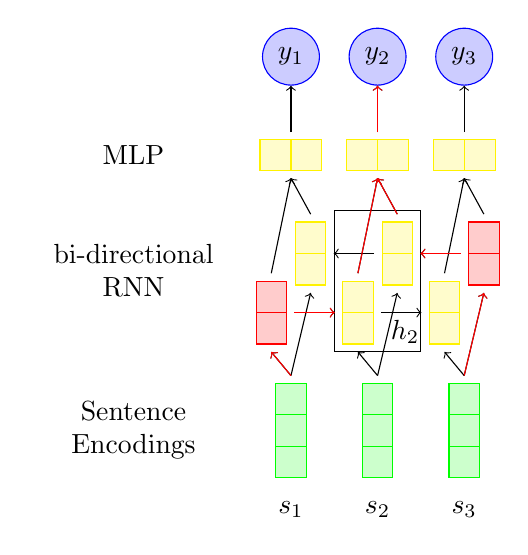
\begin{tikzpicture}[
  hid/.style 2 args={
    rectangle split,
    draw=#2,
    rectangle split parts=#1,
    fill=#2!20,
    outer sep=1mm},
  mlp/.style 2 args={
    rectangle split,
    rectangle split horizontal,
    draw=#2,
    rectangle split parts=#1,
    fill=#2!20,
    outer sep=1mm}
]


\node (label1) at (-.9,-1) {\begin{tabular}{c}Sentence\\ Encodings\end{tabular}};
\node (label2) at (-.9,1) {\begin{tabular}{c}bi-directional\\ RNN\end{tabular}};
\node (label3) at (-.9,2.5) {MLP};

 \foreach \i [count=\step from 1] in {$s_1$, $s_2$, $s_3$}
    \node (i\step) at (1.1*\step, -2) {\i};
  % draw embedding and hidden layers for text input
  \foreach \step in {1,...,3} {
    \node[hid={3}{green}] (e\step) at (1.1*\step, -1) {};    
    %\draw[->] (i\step.north) -> (e\step.south);
  }

  \foreach \step in {1,...,3} {
    \node[hid={2}{yellow}] (h_f_\step) at (-.25 + 1.1 *\step, .5) {};    
    \node[hid={2}{yellow}] (h_r_\step) at (.25 + 1.1 *\step, 1.25) {};    
    \draw[->] (e\step.north) -> (h_f_\step.south);
    \draw[->] (e\step.north) -> (h_r_\step.south);
    \node[mlp={2}{yellow}] (h_\step) at (1.1 *\step, 2.5) {};    
    \node[circle, draw=blue, fill=blue!20] (y_\step) at (1.1 *\step, 3.75) {$y_\step$};    
    \draw[->] (h_\step.north) -> (y_\step.south);
    \draw[->] (h_f_\step.north) -> (h_\step.south);
    \draw[->] (h_r_\step.north) -> (h_\step.south);
  }

  \foreach \step/\steppp in {1/2, 2/3} {
    \draw[->] (h_f_\step.east) -> (h_f_\steppp.west);
    \draw[->] (h_r_\steppp.west) -> (h_r_\step.east);
  }
  \uncover<2->{
 \draw (1.65,0) rectangle (2.75,1.8); 
 \node (hlabel) at (2.55, .25) {$h_2$};
    }

    \uncover<3->{ 
    \draw[->,red] (e1.north) -> (h_f_1.south);
    \draw[->,red] (h_f_1.east) -> (h_f_2.west);
    \draw[->,red] (h_f_2.north) -> (h_2.south);
    \node[hid={2}{red}] (h_f_1) at (-.25 + 1.1 *1, .5) {};    
}

\uncover<4->{
    \draw[->,red] (h_r_3.west) -> (h_r_2.east);
    \draw[->,red] (h_r_2.north) -> (h_2.south);
    \draw[->,red] (h_2.north) -> (y_2.south);
    \draw[->,red] (e3.north) -> (h_r_3.south);
    \node[hid={2}{red}] (h_r_3) at (.25 + 1.1 *3, 1.25) {};    
}

\end{tikzpicture}

%    \end{column}
%    \begin{column}{0.5\textwidth}
%      \uncover<2->{
%            $p(y|h) = \prod_{i=1}^n p(y_i|h)$ 
%      }
%    \end{column}
%  \end{columns}
%\end{frame}
%
%\begin{frame}{Sentence Extractor}
%  \textbf{Previous Work}\\~\\
%  ~~ -- \textbf{Cheng and Lapata Extractor} ~~ seq2seq inspired architecture 
%                                               (Cheng and Lapata, 2016)\\
%  ~~ -- \textbf{SummaRunner Extractor} ~~ RNN inspired architecture with 
%                                          document and summary representations 
%                                          (Nallapati et al., 2016)\\
%  ~\\~\\
%  \textbf{Our Extractors}\\~\\
%  ~~ -- \textbf{RNN Extractor} ~~ Simplified version of SummaRunner \\
%  ~~ -- \alert{\textbf{Seq2Seq Extractor}} ~~ seq2seq (with attention) inspired
%                                              architecture \\
%\end{frame}
%
%
%
%\begin{frame}{Seq2Seq Extractor}
%    \begin{columns}
%        \begin{column}{0.5\textwidth}
%            
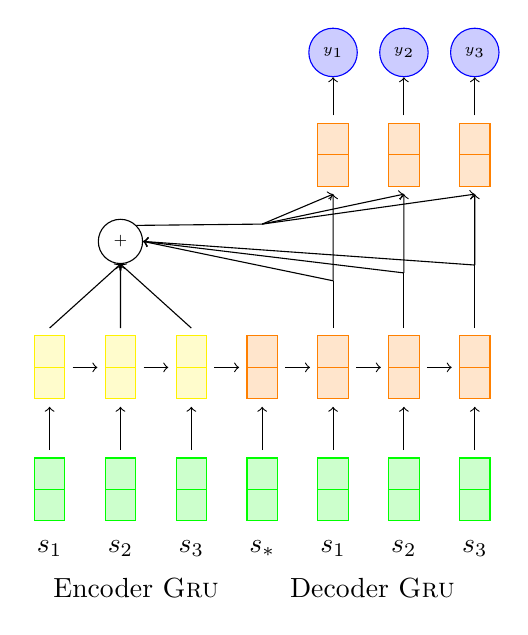
\begin{tikzpicture}[
  hid/.style 2 args={
    rectangle split,
    draw=#2,
    rectangle split parts=#1,
    fill=#2!20,
    outer sep=1mm},
  mlp/.style 2 args={
    rectangle split,
    rectangle split horizontal,
    draw=#2,
    rectangle split parts=#1,
    fill=#2!20,
    outer sep=1mm}
]


  \foreach \i [count=\step from 1] in {$s_1$, $s_2$, $s_3$} {
    \node (i\step) at (.9*\step, -1.5) {\i};
    \node[hid={2}{green}] (e\step) at (.9*\step, -.75) {};    
  }
  \node (i4) at (.9*4, -1.5) {$s_*$};

  
  \node[hid={2}{green}] (e4) at (.9*4, -.75) {};    
  \foreach \i [count=\step from 5] in {$s_1$, $s_2$, $s_3$} {
    \node (i\step) at (.9*\step, -1.5) {\i};
    \node[hid={2}{green}] (e\step) at (.9*\step, -.75) {};    
  }

  \node (enclbl) at (2,-2) {Encoder \textsc{Gru}};
  \node (enclbl) at (5,-2) {Decoder \textsc{Gru}};
%?
  \foreach \step in {1,...,3} {
%?    \node[hid={2}{yellow}] (h_r_\step) at (-.25 + .9 *\step, .5) {};    
    \node[hid={2}{yellow}] (h_f_\step) at (.9 *\step, .8) {};    
    \draw[->] (e\step.north) -> (h_f_\step.south);
%?    \draw[->] (e\step.north) -> (h_r_\step.south);
%?%    \node[mlp={2}{yellow}] (h_\step) at (.9 *\step, 2.5) {};    
%?%    \node[circle, draw=blue, fill=blue!20] (y_\step) at (.9 *\step, 3.75) {$y_\step$};    
%?%    \draw[->] (h_\step.north) -> (y_\step.south);
%?%    \draw[->] (h_f_\step.north) -> (h_\step.south);
%?%    \draw[->] (h_r_\step.north) -> (h_\step.south);
  }
%?
%  \foreach \step in {5,...,8} {
%?    \node[hid={2}{orange}] (h_r_\step) at (-.25 + .9 *\step, .5) {};    
%?    \draw[->] (e\step.north) -> (h_r_\step.south);
%?  }
  \foreach \step in {4,...,7} {
    \node[hid={2}{orange}] (h_f_\step) at (.9 *\step, .8) {};    
    \draw[->] (e\step.north) -> (h_f_\step.south);
%?%    \draw[->] (e\step.north) -> (h_r_\step.south);
%?%    \node[mlp={2}{yellow}] (h_\step) at (.9 *\step, 2.5) {};    
%?%    \node[circle, draw=blue, fill=blue!20] (y_\step) at (.9 *\step, 3.75) {$y_\step$};    
%?%    \draw[->] (h_\step.north) -> (y_\step.south);
%?%    \draw[->] (h_f_\step.north) -> (h_\step.south);
%?%    \draw[->] (h_r_\step.north) -> (h_\step.south);

  }
%?
  \draw[->] (h_f_1.east) -> (h_f_2.west);
  \draw[->] (h_f_2.east) -> (h_f_3.west);
  \draw[->] (h_f_3.east) -> (h_f_4.west);
  \draw[->] (h_f_4.east) -> (h_f_5.west);
  \draw[->] (h_f_5.east) -> (h_f_6.west);
  \draw[->] (h_f_6.east) -> (h_f_7.west);
%? 
%?  \draw[->] (h_r_3.west) -> (h_r_2.east);
%?  \draw[->] (h_r_2.west) -> (h_r_1.east);
%?  \node (lborder) at (-.25 + .9 * 0, .5) {};
%?  \node (rborder) at (-.1 + .9 * 9, .5) {};
%?  \draw[->,dashed] (h_r_1.west) -- (lborder);
%?  \draw[->,dashed] (rborder) -- (h_r_8.east);
%?  \draw[->] (h_r_8.west) -> (h_r_7.east);
%?  \draw[->] (h_r_7.west) -> (h_r_6.east);
%?  \draw[->] (h_r_6.west) -> (h_r_5.east);
%?
  \node[circle,draw=black] (attn1) at (1.8, 2.4) {\tiny$+$};    
% \node[circle,draw=black] (attn2) at (4, 2.6) {\tiny$+$};    
% \node[circle,draw=black] (attn3) at (6, 2.6) {\tiny$+$};    
  
  \uncover<2->{\node[hid={2}{orange}] (h1) at (4.5, 3.5) {};
  \node[circle, draw=blue, fill=blue!20] (y1) at (4.5, 4.8) {\tiny $y_1$};}
  \uncover<3->{\node[hid={2}{orange}] (h2) at (5.4, 3.5) {};
  \node[circle, draw=blue, fill=blue!20] (y2) at (5.4, 4.8) {\tiny $y_2$}; }   
  \uncover<4->{\node[hid={2}{orange}] (h3) at (6.3, 3.5) {};
  \node[circle, draw=blue, fill=blue!20] (y3) at (6.3, 4.8) {\tiny $y_3$};}


%?
  \foreach \step in {1,...,3} {
    %  \node (m\step) at (\step * .9, 1.9) {};
      \path[draw=black,->] (h_f_\step.north) -- (attn1.south);
      %\path[draw=black,-] (h_r_\step.north) -- (m\step.center);
    %  \foreach \stepj in {1,...,1} {
    %      \path[draw=black,->] (m\step.center) -- (attn\stepj.south);
    %  } 
  }
%?
      \node (apt) at (3.6, 2.62) {};
      \uncover<2->{\path[draw=black,-] (attn1.north east) -- (apt.center);}
      \uncover<2->{\path[draw=black,->] (apt.center) -- (h1.south);}
      \uncover<3->{\path[draw=black,->] (apt.center) -- (h2.south);}
      \uncover<4->{\path[draw=black,->] (apt.center) -- (h3.south);}
      \uncover<2->{\path[draw=black,->] (h1.north) -- (y1.south);}
      \uncover<3->{\path[draw=black,->] (h2.north) -- (y2.south);}
      \uncover<4->{\path[draw=black,->] (h3.north) -- (y3.south);}

      \uncover<2->{
  \node (m21) at (5* .9, 1.9) {};
  \path[draw=black,-] (h_f_5.north) -- (m21.center);
  \path[draw=black,->] (m21.center) -- (attn1.east);
  \path[draw=black,->] (m21.center) -- (h1.south);
}

  \uncover<3->{
  \node (m22) at (6* .9, 2) {};
  \path[draw=black,-] (h_f_6.north) -- (m22.center);
  \path[draw=black,->] (m22.center) -- (attn1.east);
  \path[draw=black,->] (m22.center) -- (h2.south);
  }
  \uncover<4->{
  \node (m23) at (7* .9, 2.1) {};
  \path[draw=black,-] (h_f_7.north) -- (m23.center);
  \path[draw=black,->] (m23.center) -- (attn1.east);
  \path[draw=black,->] (m23.center) -- (h3.south);
}



\end{tikzpicture}



%        \end{column}
%        \begin{column}{0.5\textwidth}
%            \begin{align*}
%                p(y|h) &= \prod_{i=1}^n p(y_i|h)\\
%                p(y_i|h) &= \sigma\left(W \left[ \begin{array}{l} h_i^{(d)}\\
%         \tilde{h}_i \end{array} \right]    + b \right) \\
%         \tilde{h}_i & = \sum_{j=1}^{n} \alpha_{i,j} \cdot h^{(e)}_j\\
%         \alpha_{i,j} & = \operatorname{Softmax}(h^{(e)}  \cdot h^{(d)}_i)_j \\
%            & \propto \exp\left(h^{(e)}_j  \cdot h^{(d)}_i \right) \\
%            \end{align*}
%        \end{column}
%    \end{columns}
%\end{frame}
%
%\begin{frame}{Cheng \& Lapata Extractor}
%  \begin{columns}
%    \begin{column}{0.5\textwidth}
%        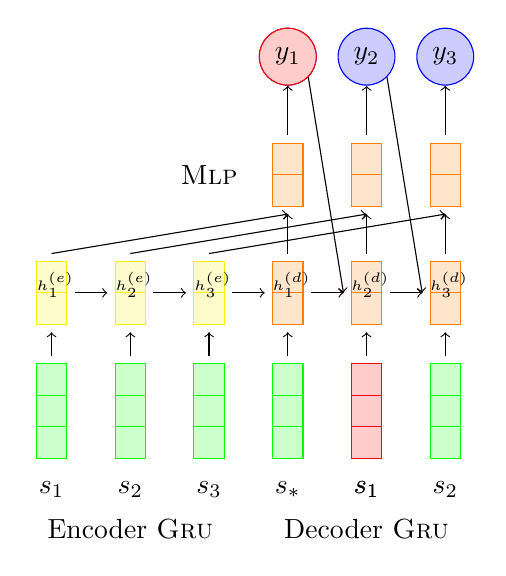
\begin{tikzpicture}[
  hid/.style 2 args={
    rectangle split,
    draw=#2,
    rectangle split parts=#1,
    fill=#2!20,
    outer sep=1mm},
  mlp/.style 2 args={
    rectangle split,
    rectangle split horizontal,
    draw=#2,
    rectangle split parts=#1,
    fill=#2!20,
    outer sep=1mm}
]

 \foreach \i [count=\step from 1] in {$s_1$, $s_2$, $s_3$, $s_*$, $s_1$, $s_2$}
    \node (i\step) at (1*\step, -2) {\i};
  % draw embedding and hidden layers for text input
  \foreach \step in {1,...,3} {
    \node[hid={3}{green}] (e\step) at (1*\step, -1) {};    
  }
    \node[hid={3}{green}] (e4) at (1*4, -1) {};    
  \foreach \step in {5,...,6} {
    \node[hid={3}{green}] (e\step) at (1*\step, -1) {};    
  }

  \foreach \step in {1,...,3} {
    \node[hid={2}{yellow}] (h_f_\step) at (1 *\step, .5) {};    
    \draw[->] (e\step.north) -> (h_f_\step.south);
  }

  \foreach \step in {1,...,3} {
      \node (hlbl\step) at (1*\step + .05, .6) {\tiny $h^{(e)}_\step$};    
  }


  \foreach \step in {4,...,6} {
    \node[hid={2}{orange}] (h_f_\step) at (1 *\step, .5) {};    
    \node[hid={2}{orange}] (g_f_\step) at (1 *\step, 2) {};    
    \draw[->] (e\step.north) -> (h_f_\step.south);
  }

  \foreach \step in {1,...,3} {
      \node (hlbl\step) at (1*\step + 3 + .05, .6) {\tiny $h^{(d)}_\step$};    
  }
  \foreach \step in {1,...,3} {
    \node[circle, draw=blue, fill=blue!20] (y_\step) at (3 + 1 *\step, 3.5) {$y_\step$};    
 }
    \draw[->] (y_1.south east) -> (h_f_5.west);
    \draw[->] (y_2.south east) -> (h_f_6.west);
    \draw[->] (h_f_4.north) -> (g_f_4.south);
    \draw[->] (g_f_4.north) -> (y_1.south);
    \draw[->] (h_f_5.north) -> (g_f_5.south);
    \draw[->] (g_f_5.north) -> (y_2.south);
    \draw[->] (h_f_6.north) -> (g_f_6.south);
    \draw[->] (g_f_6.north) -> (y_3.south);
 \foreach \step/\steppp in {1/2, 2/3, 3/4, 4/5, 5/6} {
   
    \draw[->] (h_f_\step.east) -> (h_f_\steppp.west);
  }
    \draw[->] (h_f_1.north) -> (g_f_4.south);
    \draw[->] (h_f_2.north) -> (g_f_5.south);
    \draw[->] (h_f_3.north) -> (g_f_6.south);

    \node (enc) at (2,-2.5) {Encoder \textsc{Gru}};
    \node (dec) at (5,-2.5) {Decoder \textsc{Gru}};
    \node (mlp) at (3, 2) {\textsc{Mlp}};

  \uncover<5->{
  \node (i5) at (1*5, -2) {\alert{$s_1$}};
    \node[circle, draw=red, fill=red!20] (y_1) at (3 + 1 *1, 3.5) {$y_1$};    
    \node[hid={3}{red}] (e5) at (1*5, -1) {};    
}

\end{tikzpicture}

%    \end{column}
%    \begin{column}{0.5\textwidth}
%      \begin{align*}
%        \uncover<1->{p(y|h) &= \prod_{i=1}^n p(y_i|y_{<i}, h^{(d)}_{<i}, 
%                                                       h^{(e)} )}\\
%        \uncover<2->{p_i & \triangleq p(y_i=1|h) = 
%                            \textsc{Mlp}([h^{(e)}_i; h^{(d)}_i])}\\
%        \uncover<3->{h^{(d)}_i &= \textsc{Gru}\left(h_{i-1}^{(d)},  
%                                 \alert<5->{p_{i-1} \cdot  s_{i-1}}\right)}
%      \end{align*}
%    \end{column}
%  \end{columns}
%\end{frame}
%
%\begin{frame}{Sentence Extractor}
%  \textbf{Previous Work}\\~\\
%  ~~ -- \textbf{Cheng and Lapata Extractor} ~~ seq2seq inspired architecture 
%                                               (Cheng and Lapata, 2016)\\
%  ~~ -- \alert{\textbf{SummaRunner Extractor}} ~~ RNN inspired architecture 
%                                                  with document and summary 
%                                                  representations 
%                                                  (Nallapati et al., 2016)\\
%  ~\\~\\
%  \textbf{Our Extractors}\\~\\
%  ~~ -- \textbf{RNN Extractor} ~~ Simplified version of SummaRunner \\
%  ~~ -- \textbf{Seq2Seq Extractor} ~~ seq2seq (with attention) inspired 
%                                      architecture \\
%\end{frame}
%
%
%
%\begin{frame}{SummaRunner Extractor}
%  \begin{columns}
%    \begin{column}{0.5\textwidth}
%      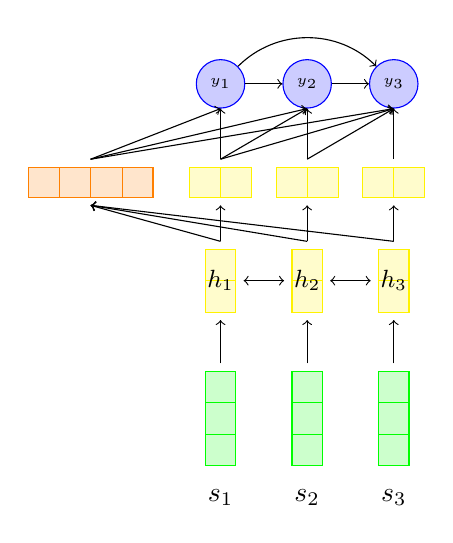
\begin{tikzpicture}[
  hid/.style 2 args={
    rectangle split,
    draw=#2,
    rectangle split parts=#1,
    fill=#2!20,
    outer sep=1mm},
  mlp/.style 2 args={
    rectangle split,
    rectangle split horizontal,
    draw=#2,
    rectangle split parts=#1,
    fill=#2!20,
    outer sep=1mm}
]

 \foreach \i [count=\step from 1] in {$s_1$, $s_2$, $s_3$}
 \node (i\step) at (1.1*\step, -1.5) {\i};
  % draw embedding and hidden layers for text input
  \foreach \step in {1,...,3} {
    \node[hid={3}{green}] (e\step) at (1.1*\step, -.5) {};    
  }

        \node[mlp={4}{orange}] (h_0) at (1.1 *-.5, 2.5) {};    
  \foreach \step in {1,...,3} {
    \node[hid={2}{yellow}] (h_f_\step) at (1.1 *\step, 1.25) {};    
    \node (lblh_f_\step) at (1.1 *\step, 1.25) {\small $h_\step$};    
    \draw[->] (h_f_\step.north) -> (h_0.south);
    \draw[->] (e\step.north) -> (h_f_\step.south);
    \node[mlp={2}{yellow}] (h_\step) at (1.1 *\step, 2.5) {};    
    \node[circle, draw=blue, fill=blue!20] (y_\step) at (1.1 *\step, 3.75) {\tiny $y_\step$};    
    \draw[->] (h_\step.north) -> (y_\step.south);
    \draw[->] (h_f_\step.north) -> (h_\step.south);
    %\draw[->] (h_r_\step.north) -> (h_\step.south);
  }

  \foreach \step/\steppp in {1/2, 2/3} {
    \draw[<->] (h_f_\step.east) -> (h_f_\steppp.west);
    %\draw[->] (h_r_\steppp.west) -> (h_r_\step.east);
  }
 
    \draw[->] (h_0.north) -> (y_1.south);
    \draw[->] (h_0.north) -> (y_2.south);
    \draw[->] (h_0.north) -> (y_3.south);
    \draw[->] (y_1.east) -> (y_2.west);
    \draw[->] (y_2.east) -> (y_3.west);
    \draw[->] (h_1.north) -> (y_2.south);
    \draw[->] (h_1.north) -> (y_3.south);
    \draw[->] (h_2.north) -> (y_3.south);
    \draw [bend left=45,->] (y_1) to (y_3);
\end{tikzpicture}

%    \end{column}
%    \begin{column}{0.5\textwidth}
%      $d = \tanh\big(b_d + W_d \frac{1}{n} \sum_{i=1}^n h_i   \big) $\\
%      $ g_i  = \sum_{j=1}^{i-1} p(y_j=1|y_{<j},h) \cdot h_j$\\
%      \begin{align*}
%        \textit{content}  \quad a^{(con)}_i & =W^{(con)} h_i \\
%        \textit{salience} \quad a^{(sal)}_i & = h_i^TW^{(sal)} d \\
%        \textit{novelty} \quad a^{(nov)}_i & = -h_i^TW^{(nov)} \tanh(g_i) 
%                    \label{eq:srnov} \\
%        \textit{position} \quad a^{(pos)}_i & = W^{(pos)} l_i \\
%        \textit{quartile} \quad a^{(qrt)}_i & = W^{(qrt)} r_i
%      \end{align*}
%      $p(y_i|y_{<i}, h) = \sigma\left(\begin{array}{l} a^{(con)}_i 
%        +a^{(sal)}_i + a^{(nov)}_i+ \\ a^{(pos)}_i + a^{(qrt)}_i + 
%         b \end{array}\right) $ \\
%    \end{column}
%  \end{columns}
%\end{frame}




\section{Data}

\begin{frame}{Datasets - News}
  \begin{center}
    \begin{tabular}{ rfrfr }
      \toprule
      \textbf{Dataset} & \textbf{Train} & \textbf{Valid} & \textbf{Test} &
        \textbf{Refs} \\
        \midrule
        CNN/DailyMail & 287,113 & 13,368 & 11,490 & 1\\
        NYT & 44,382 & 5,523 & 6,495 & 1.93\\
        DUC 2001/2002 & 516 & 91 & 657 & 2 \\
      \bottomrule
    \end{tabular}
  \end{center} 
  ~\\

  Sizes of the training, validation, test splits for each dataset
  and the average number of test set human reference summaries per document.

\end{frame}

\begin{frame}{Datasets - Personal Narratives/Office Meetings/Medical Journal Articles}
  \begin{center}
    \begin{tabular}{ rfrfr }
      \toprule
      \textbf{Dataset} & \textbf{Train} & \textbf{Valid} & \textbf{Test} &
        \textbf{Refs} \\
        \midrule
      Reddit & 404 & 24 & 48 & 2 \\
      AMI & 98 & 19 & 20 & 1 \\
      PubMed & 21,250 & 1,250 & 2,500 & 1\\
      \bottomrule
    \end{tabular}
  \end{center} 
  ~\\

  Sizes of the training, validation, test splits for each dataset
  and the average number of test set human reference summaries per document.

  \begin{itemize}
      \item \textbf{Reddit} -- personal narratives (Ouyang et al. 2017)
      \item \textbf{AMI} -- Work place meeting summarization  \\
     \item \textbf{PubMed} -- a random sample of journal articles from the PMC Open Access subset.  \\
  \end{itemize}

\end{frame}


\section{Experiments}

\begin{frame}{Experiments}
%
    \alert<4>{\textbf{Main Experiment}}\\
    Evaluate encoder/extractor pairs using ROUGE-2 recall.\\
%
  \begin{columns}
    \begin{column}{0.3\textwidth}
    \uncover<5->{\textbf{Additional Experiments}}    
      \begin{itemize}
        \uncover<5->{\item \alert<5>{fine-tuned embeddings}}
        \uncover<6->{\item \alert<6>{word class ablations}}
        \uncover<7->{\item \alert<7>{sentence order shuffling}}
      \end{itemize}
    \end{column}
    \begin{column}{0.7\textwidth}
        \input{5_experiments/emb_experiments_pic.tex} 
    \end{column}
  \end{columns}
\end{frame}

\begin{frame}{Model Training}

    Maximum Likelihood training using gold extract summaries.

    \[\max_{\theta} \frac{1}{|\mathcal{D}|} \sum_{(s,y^*)\in \mathcal{D}} 
    \log p(y^*| s) \]

   
    ~\\

    Gold extract summaries $y^*$ created by greedily selecting the sentences that maximizing ROUGE, as in Nallapati et al. (2016).

\end{frame}

\begin{frame}{Summary Generation}

    \begin{enumerate}
        \item Rank sentences $s_i$ in decreasing order by $p(y_i=1|h)$.
        \item Create a summary by extracting the top ranked sentences until a word length budget.
    \end{enumerate}

\end{frame}


\section{Results}


\begin{frame}{Choice of Sentence Encoder: News}
  \begin{center}
  \input{6_results/6_encoder_results_news.tex}    
  \end{center}
  ~\\

  Averaging is either the \alert{\textbf{best}} encoder or 
  \textbf{statistically indistinguishable} from the best encoder!

\end{frame}

\begin{frame}{Choice of Sentence Encoder: Non-News}
  \begin{center}
    \input{6_results/6_encoder_results_nonnews.tex}    
  \end{center}
  ~\\

  Averaging is either the \alert{\textbf{best}} encoder or 
  \textbf{statistically indistinguishable} from the best encoder!
\end{frame}

\begin{frame}{Choice of Sentence Extractor: News}
    
 \begin{center}
   \input{6_results/6_extractor_results_news.tex}
 \end{center}
 
 ~\\

 \textsc{Seq2Seq} is the \alert{\textbf{best}} or \textbf{statistically 
 indistinguishable} from the best system.

 ~\\
 \textsc{Rnn} extractor as good as \textsc{SummaRunner} or 
 \textsc{Cheng \& Lapata} extractors on CNN/DailyMail data.

  

\end{frame}

\begin{frame}{Choice of Sentence Extractor: Non-News}
    
 \begin{center}
   \input{6_results/6_extractor_results_nonnews.tex}
 \end{center}

 ~\\

 \textsc{Seq2Seq} is the \alert{\textbf{best}} or statistically indistinguishable from the best
 system.


\end{frame}



\begin{frame}{Word Embedding Fine-Tuning: (News)}
  \begin{center}
    \begin{tabular}{ccccc}
 & & \multicolumn{3}{c}{\textbf{Rouge-2 Recall}}\\
      \toprule
        \textbf{Ext} & \textbf{Emb}  & 
           \textbf{CNN/DM} & 
           \textbf{NYT} & 
           \textbf{DUC} \\
      \midrule
      \multirow{2}{*}{\textsc{Seq2Seq}} 
        & Fixed & \textbf{25.6} & \textbf{35.7} & \textbf{22.8} \\
        & Fine-Tuned &         25.3  & \textbf{35.7} & \textbf{22.9} \\
      \hline
      \multirow{2}{*}{\textsc{Cheng \& Lapata}} 
        & Fixed & \textbf{25.3} & \textbf{35.6} & \textbf{23.1} \\
        & Fine-Tuned &         24.9  &         35.4  & \textbf{23.0} \\
      \bottomrule
  \end{tabular}
 \end{center}

 ~\\
 
 Performance difference when using \textit{fixed} embeddings versus 
 \textit{fine-tuned} embeddings.
 
  ~\\

  Models are using the \textsc{Avg} encoder and are initialized with 
  Glove embeddings. 

  ~\\

  \textbf{No statistically significant improvement} on news with fine-tuning!

\end{frame}

\begin{frame}{Word Embedding Fine-Tuning: Non-News}
 \begin{center}
  \begin{tabular}{ccccc}
   \toprule
   \textbf{Ext} & \textbf{Emb}  & 
        \textbf{Reddit} & \textbf{AMI} & \textbf{PubMed} \\
   \midrule
   \multirow{2}{*}{\textsc{Seq2Seq}}
      & Fixed & \textbf{13.6} &         5.5  & \textbf{17.7} \\
      & Fine-Tuned & \textbf{13.8} & \textbf{5.8} &         16.9  \\
   \hline
   \multirow{2}{*}{\textsc{Cheng \& Lapata}} 
      & Fixed & \textbf{13.6} & \textbf{6.1} & \textbf{17.7} \\
      & Fine-Tuned & \textbf{13.4} & \textbf{6.2} & \textbf{16.4} \\
   \bottomrule
  \end{tabular}
 \end{center}

 ~\\
 
 Performance difference when using \textit{fixed} embeddings versus 
 \textit{fine-tuned} embeddings.
 
 ~\\

 All models are using the \textsc{Avg} encoder and are initialized with 
 pretrained Glove embeddings from gigaword/wikipedia. 

 ~\\
 \textbf{Statistically significant improvement} with \textsc{Seq2Seq} on AMI
 data.\\
 Otherwise, same trend as news, no improvement using fine-tuning.

\end{frame}

\begin{frame}{Word Class Ablation: ROUGE-2 Recall}
 \begin{center}
  \begin{tabular}{lcccccc}
   \toprule
   \multirow{1}{*}{\textbf{Ablation}} & 
            \textbf{CNN/DM} & \textbf{NYT} & \textbf{DUC} &
            \textbf{Reddit} & \textbf{AMI} & \textbf{PubMed} \\
   \midrule
     All Words & $\mathbf{25.4}$ & $\mathbf{34.7}$ & $22.7$ &
                  $\mathbf{11.4}$ & $5.5$ & $\mathbf{17.0}$  \\
     $-$ Nouns & $25.3^\dagger$  & $34.3^\dagger $ & $22.3^\dagger$  &
   $10.3^\dagger$ & \alert<3>{$3.8^\dagger$} & \alert<3>{$15.7^\dagger$} \\
     $-$ Verbs & $25.3^\dagger$  & $34.4^\dagger $ & $22.4^\dagger$ &
            $10.8$ & $5.8$ & $16.6^\dagger$ \\
 $-$ Adj/Adv & 
  $25.3^\dagger$ & $34.4^\dagger$ & $22.5$ &
   \alert<4>{$9.5^\dagger$} & $5.4$ & $16.8^\dagger$ \\
   $-$ Function & $25.2^\dagger$ & $34.6^\dagger$ & \alert<2>{$\mathbf{22.9}^\dagger$} &
   $10.3^\dagger$ & \alert<2>{$\mathbf{6.3}^\dagger$} & $16.6^\dagger$ \\
   \bottomrule
  \end{tabular}
 \end{center}

 ~\\

 RNN extractor with Averaging encoder. 

 ~\\

 \textbf{Bold} is best performance. $\dagger$ indicates significant 
 difference from All Words, i.e. non-ablated model.

 ~\\



\end{frame}



\begin{frame}{Shuffled vs In-Order (News)}

 \begin{center}
  \begin{tabular}{ccL{2cm}m{1cm}L{.75cm}} 
   \toprule
   \textbf{Ext.} & \textbf{Order} & 
                           \textbf{CNN/DM} & \textbf{NYT} & \textbf{DUC} \\
   \midrule
%?   \multirow{2}{*}{RNN} 
%?       & In-Order & 
%?       \textbf{25.4} & \textbf{34.7} & \textbf{22.7} \\
%?       & Shuffled & 
%?               22.8 &          25.0  &         18.2  \\
   \hline
   \multirow{2}{*}{Seq2Seq}
       & In-Order & 
       \textbf{25.6} & \textbf{35.7} &  \textbf{22.8} \\
       & Shuffled & 
               21.7  &         25.6  &          21.2  \\
   \bottomrule
  \end{tabular}
 \end{center}

 ~\\

 Shuffled model is trained on shuffled sentence order documents.

 ~\\

 Both models evaluated on in-order data.

\end{frame}

\begin{frame}{Shuffled vs In-Order (Other)}

 \begin{center}
  \begin{tabular}{ccccc} 
   \toprule
   \textbf{Ext.} & \textbf{Order} & 
                           \textbf{Reddit} & \textbf{AMI} & \textbf{PubMed} \\
   \midrule
   \multirow{2}{*}{Seq2Seq}
       & In-Order & 
       \textbf{13.6} &         5.5  &  \textbf{17.7} \\
       & Shuffled & 
       \textbf{13.5} & \textbf{6.0} &          14.9  \\
   \bottomrule
  \end{tabular}
 \end{center}

 ~\\

 Shuffled model is trained on shuffled sentence order documents.

 ~\\

 Both models evaluated on in-order data.

\end{frame}



\begin{frame}

    Summary of Findings:
    \begin{itemize}
        \item<1-> Simpler is good enough:
            \begin{itemize}
        \item<2-> Averaging sentence encoder is as good as RNNs or CNNs.
        \item<3-> \textsc{Seq2Seq} extractor on par with more complicated models, as is \textsc{Rnn} in many cases.
    \end{itemize}
        \item<4-> Richer features are needed.
    \begin{itemize}
        \item<5-> Sentence salience not fully captured by word embeddings/shallow lexical semantics
        \item<6-> Sentence position dominates the learning signal. 
    \end{itemize}
    \end{itemize}

    \uncover<8->{

~\\

~\\

        \textbf{Thank you for listening! Ask me questions!}


        ~\\
        Code and data at: \url{https://github.com/kedz/nnsum/tree/emnlp18-release} \\
        or \url{http://cs.columbia.edu/\~kedzie}

    }


\end{frame}



\end{document} 
